\documentclass[handout]{beamer} % or [10pt]
\setbeamertemplate{navigation symbols}{}
\usetheme{Warsaw}

% Umlaute-Encoding und Standardschrift einstellen
\usepackage[ngerman]{babel}
\usepackage[utf8]{inputenc}
\usepackage[T1]{fontenc}
\usepackage{lmodern}

\usepackage{times}
\usepackage{amsfonts,amsmath,amssymb,amsthm}

\beamersetuncovermixins{\opaqueness<1>{25}}{\opaqueness<2->{15}}

\graphicspath{{./img/}}

\title{Beamer Class Warsaw}  
\author{Jonas Berger}
\date{\today} 

\begin{document}
	
	\begin{frame}
		\titlepage
	\end{frame} 
	
	\begin{frame}
		\frametitle{Inhaltsverzeichnis}\tableofcontents
	\end{frame} 
	
	
	\section{Abschnitt Nr.1} 
	\begin{frame}
		\frametitle{Titel} 
		Die einzelnen Frames sollte einen Titel haben 
	\end{frame}
	\subsection{Unterabschnitt Nr.1.1  }
	\begin{frame} 
		Denn ohne Titel fehlt ihnen was
	\end{frame}
	
	
	\section{Abschnitt Nr. 2} 
	\subsection{Listen I}
	\begin{frame}\frametitle{Aufz\"ahlung}
		\begin{itemize}
			\item Einf\"uhrungskurs in \LaTeX  
			\item Kurs 2  
			\item Seminararbeiten und Pr\"asentationen mit \LaTeX 
			\item Die Beamerclass 
		\end{itemize} 
	\end{frame}
	
	\begin{frame}\frametitle{Aufz\"ahlung mit Pausen}
		\begin{itemize}
			\item  Einf\"uhrungskurs in \LaTeX \pause 
			\item  Kurs 2 \pause 
			\item  Seminararbeiten und Pr\"asentationen mit \LaTeX \pause 
			\item  Die Beamerclass
		\end{itemize} 
	\end{frame}
	
	\subsection{Listen II}
	\begin{frame}\frametitle{Numerierte Liste}
		\begin{enumerate}
			\item  Einf\"uhrungskurs in \LaTeX 
			\item  Kurs 2
			\item  Seminararbeiten und Pr\"asentationen mit \LaTeX 
			\item  Die Beamerclass
		\end{enumerate}
	\end{frame}
	\begin{frame}\frametitle{Numerierte Liste mit Pausen}
		\begin{enumerate}
			\item  Einf\"uhrungskurs in \LaTeX \pause 
			\item  Kurs 2 \pause 
			\item  Seminararbeiten und Pr\"asentationen mit \LaTeX \pause 
			\item  Die Beamerclass
		\end{enumerate}
	\end{frame}
	
	\section{Abschnitt Nr.3} 
	\subsection{Tabellen}
	\begin{frame}\frametitle{Tabellen}
		\begin{tabular}{|c|c|c|}
			\hline
			\textbf{Zeitpunkt} & \textbf{Kursleiter} & \textbf{Titel} \\
			\hline
			WS 04/05 & Sascha Frank &  Erste Schritte mit \LaTeX  \\
			\hline
			SS 05 & Sascha Frank & \LaTeX \ Kursreihe \\
			\hline
		\end{tabular}
	\end{frame}
	
	
	\begin{frame}\frametitle{Tabellen mit Pause}
		\begin{tabular}{c c c}
			A & B & C \\ 
			\pause 
			1 & 2 & 3 \\  
			\pause 
			A & B & C \\ 
		\end{tabular} 
	\end{frame}
	
	
	\section{Abschnitt Nr. 4}
	\subsection{Bl\"ocke}
	\begin{frame}\frametitle{Bl\"ocke}
		
		\begin{block}{Blocktitel}
			Blocktext 
		\end{block}
		
		\begin{exampleblock}{Blocktitel}
			Blocktext 
		\end{exampleblock}
		
		
		\begin{alertblock}{Blocktitel}
			Blocktext 
		\end{alertblock}
	\end{frame}
	
	\section{Abschnitt Nr. 5}
	\subsection{Geteilter Bildschirm}
	
	\begin{frame}\frametitle{Zerteilen des Bildschirmes}
		\begin{columns}
			\begin{column}{6cm}
				\begin{itemize}
					\item Beamer 
					\item Beamer Class 
					\item Beamer Class Latex 
				\end{itemize}
			\end{column}
			\begin{column}{6cm}
				\begin{tabular}{|c|c|}
					\hline
					\textbf{Kursleiter} & \textbf{Titel} \\
					\hline
					Sascha Frank &  \LaTeX \ Kurs 1 \\
					\hline
					Sascha Frank & \LaTeX \ Kursreihe \\
					\hline
				\end{tabular}
			\end{column}
		\end{columns}
	\end{frame}
	
	\subsection{Bilder} 
	\begin{frame}\frametitle{Bilder in Beamer}
		\begin{figure}
			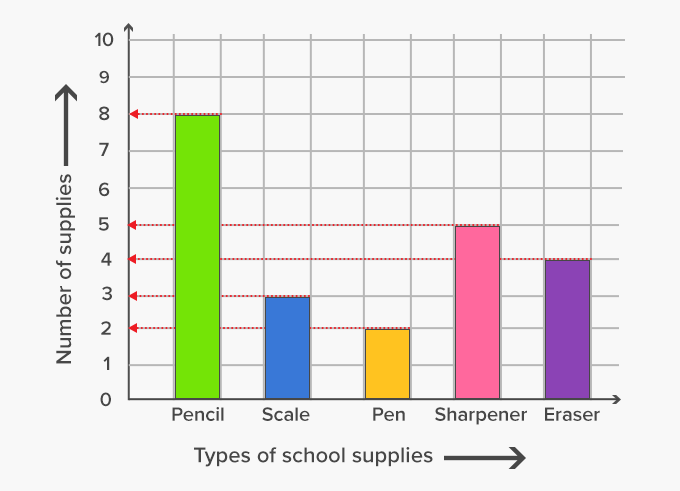
\includegraphics[scale=0.3]{PIC1} 
			\caption{Die Abbildung zeigt ein Beispielbild}
		\end{figure}
	\end{frame}
	
	
	\subsection{Bilder und Listen kombiniert} 
	
	\begin{frame}
		\frametitle{Bilder und Itemization in Beamer}
		\begin{columns}
			\begin{column}{5cm}
				\begin{itemize}
					\item<1-> Stichwort 1
					\item<3-> Stichwort 2
					\item<5-> Stichwort 3
				\end{itemize}
				\vspace{3cm} 
			\end{column}
			\begin{column}{5cm}
				\begin{overprint}
					\includegraphics<2>[scale=0.1]{PIC1}
					\includegraphics<4>[scale=0.1]{PIC2}
					\includegraphics<6>[scale=0.1]{PIC3}
				\end{overprint}
			\end{column}
		\end{columns}
	\end{frame}
	
	\subsection{Bilder die mehr Platz brauchen} 
	\begin{frame}[plain]
		\frametitle{plain, oder wie man mehr Platz hat}
		\begin{figure}
			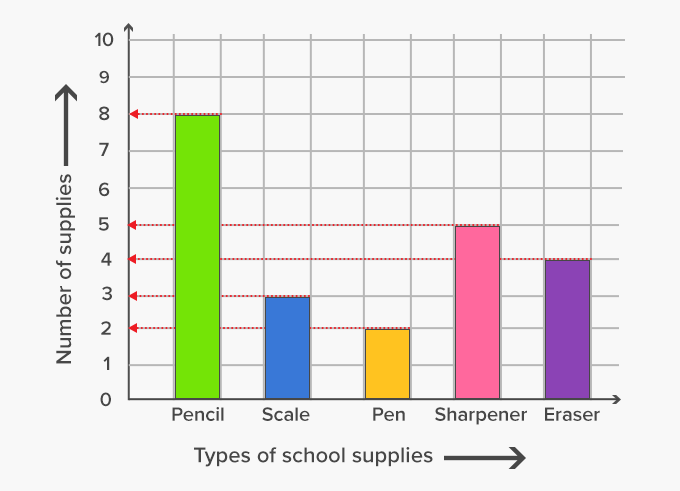
\includegraphics[scale=0.3]{PIC1} 
			\caption{Die Abbildung zeigt ein Beispielbild}
		\end{figure}
	\end{frame}
	
	
\end{document}
